% Made up for the tikra benchmark.
\usetikzlibrary{circuits.ee.IEC}
\begin{tikzpicture}[circuit ee IEC, thick, every info/.style={font=\small}]
  \draw (0,0) to [battery={info={$9\,$V}}] (0,4) -- (3,4)
        to [resistor={info={$R_1$}}] (3,2)
        to [resistor={info={$R_2$}}] (3,0) -- (0,0);
  \draw (3,2) -- (5,2) to [diode={light emitting, info'={LED}}] (5,0) -- (3,0);
  \draw (5,2) -- (7,2) to [bulb={info={lamp}}] (7,0) -- (5,0);
  \draw (0,0) -- (0,-0.4) node[ground, rotate=-90, anchor=input] {};
  \fill (3,2) circle (2pt) (5,2) circle (2pt) (3,0) circle (2pt) (5,0) circle (2pt) (0,0) circle (2pt);
  \draw[-latex, blue!60!black] (2.3,1.8) -- node[left, font=\small] {$U_2$} (2.3,0.2);
  \node[font=\footnotesize, anchor=west] at (3.6,3.6) {$U_2 = U\,\dfrac{R_2}{R_1+R_2}$};
\end{tikzpicture}
